\section{Results} % 500 words in total
\label{sec:results}

% Overview of numbers


% figure 1 - within class accuracy per model
Within-class accuracy by the model can be seen in Figure \ref{fig:wc_accuracy_x_model} (a
sister figure where scores are grouped by signature rather than by model can be found in
Appendix \ref{sec:appendixB}). We can notice some consistent patterns already. The
baseline image classification (\texttt{bic}) tends to underperform other architectures,
especially on more urban signature types. On the other hand, multi-output regression (\texttt{mor}),
using the larger chip size (32 or 64), tends to show the highest values across signature
types and models. If we look at accuracy for individual signature types, both extremes
(urbanity on one side and both countryside classes on the other)
tend to be the easiest to predict. Regarding the models, there is no immediate conclusion to be
made apart from a clear indication that the maximum probability (\texttt{maxprob}) approach is generally
worse than any of the modelling, suggesting that there is a value in the modelling step.
The within-class accuracy can be further explored using confusion matrices available as an
Appendix \ref*{sec:appendixC}.


\begin{figure}
    \centering
    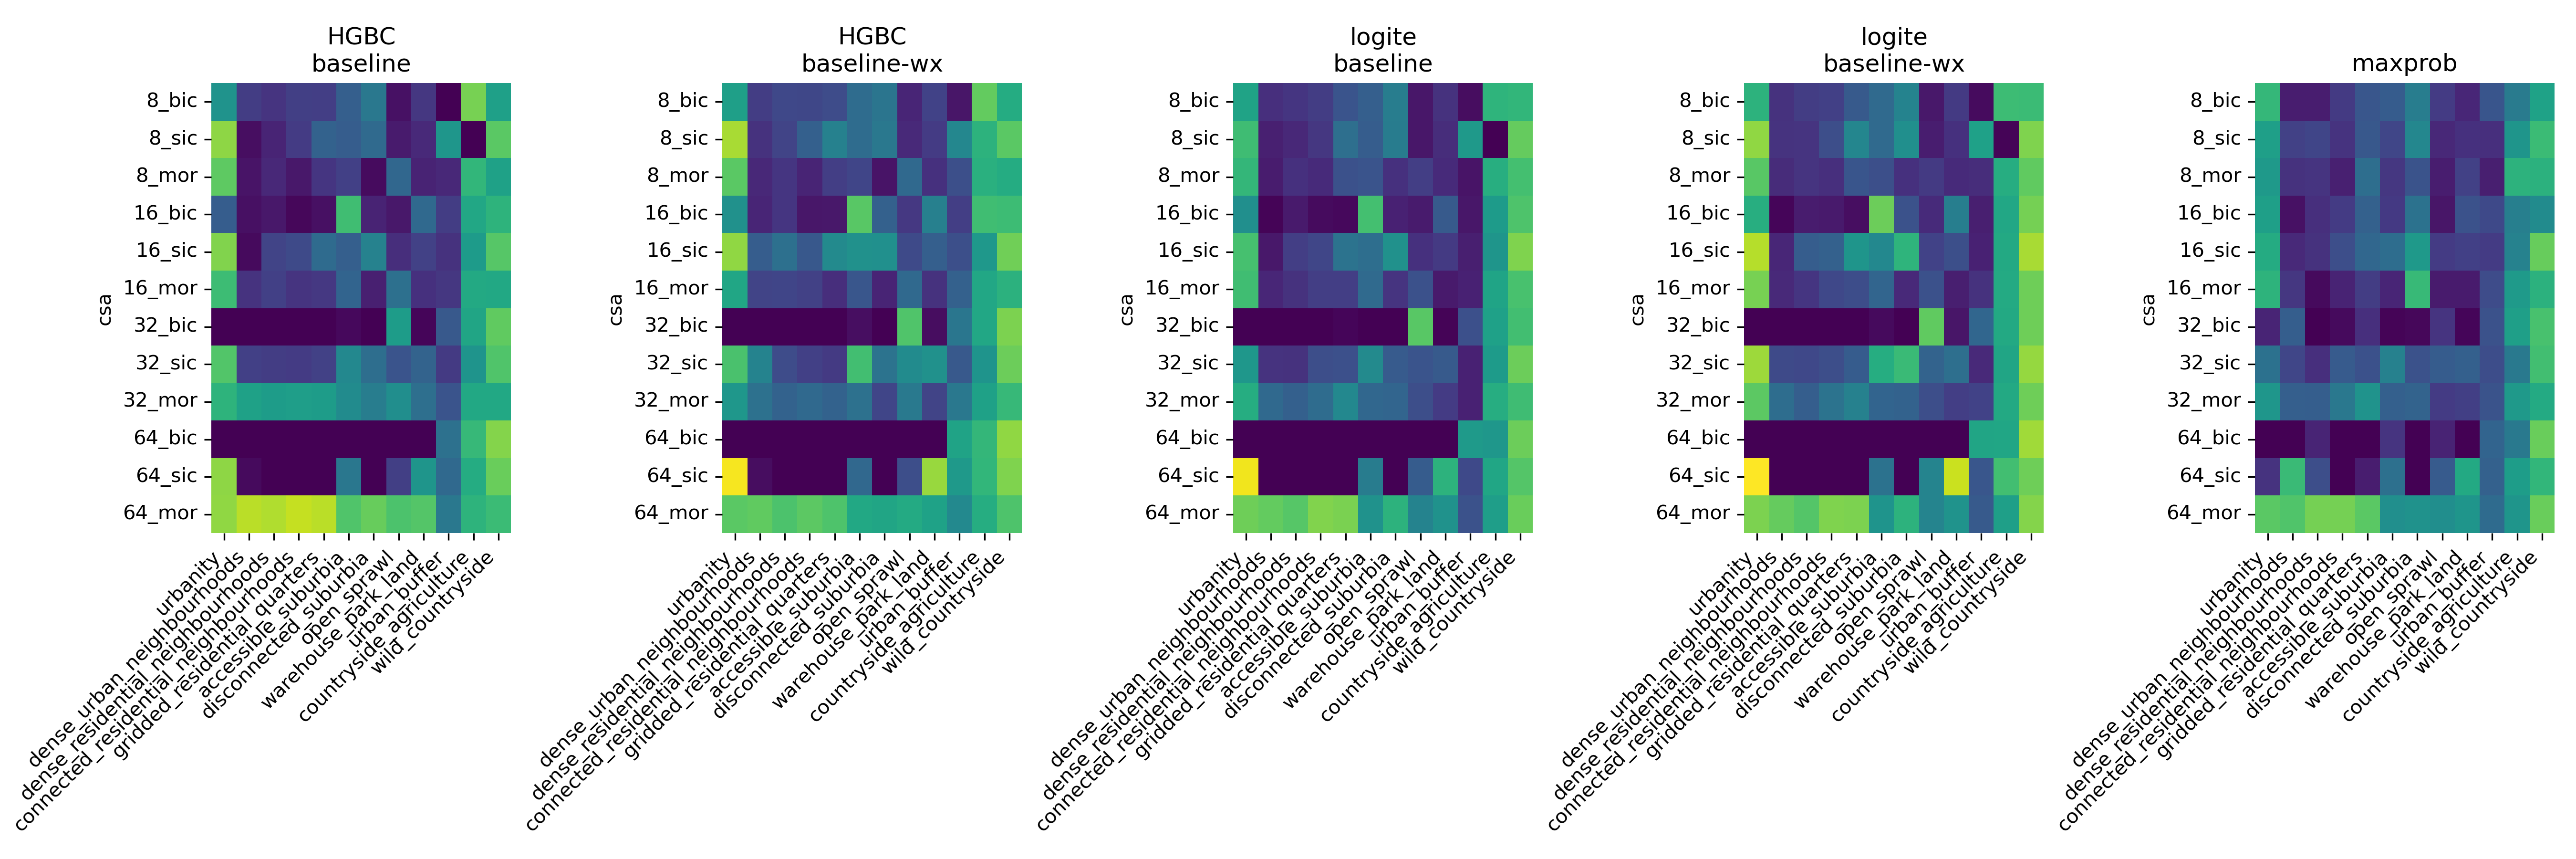
\includegraphics[width=1.0\linewidth]{fig/wc_accuracy_x_model.png}
    \caption{\footnotesize Within-class accuracy scores grouped by model. Each panel
    represents results from one of the five models compared, namely:
    histogram-based boosted classifier (\texttt{HGBC}) with features
    pertaining only to a given chip (\texttt{baseline}) or including also features
    from neighbouring ones (\texttt{baseline-wx}); Logit ensemble
    (\texttt{logite}) with the same two variations; and a simpler maximum
    probability approach (\texttt{maxprob}). Each row in the heatmap
    corresponds to a pair of chipsize (8, 16, 32, and 64 pixels)
    and architechture (baseline image classification, or \texttt{bic}; sliding
            image classification, or \texttt{sic}; and multi-output
    regression, or \texttt{mor}) used in the neural network stage of the
    pipeline. Colouring is standardised across panels and values range from
    0 (dark purple) to 1 (bright yellow).}
    \label{fig:wc_accuracy_x_model}
\end{figure}

Whilst plotting the accuracy is a way to build an intuition about the performance of
individual options, it does not quantify their effects. The linear regressions shown in
tables \ref{tab:non_sp_reg} and \ref{tab:non_sp_reg_wc} provide a better insight. The
first regression explains global performance scores (Cohen's kappa, Global Accuracy, Marco F1
weighted and Macro F1 average). We can draw a few conclusions from this. First, the chip size
seems to have a positive effect on the results, as it is consistently
significant across all metrics. Except for the average macro F1 score, there is a
positive effect of the inclusion of spatial lag in the modelling step (W). Regarding the
CNN step, we do not see a lot of significance but there are indications that sliding
image classification and multi-output regression approaches outperform baseline image
classification. Comparing the probability modelling step, we see an indication that the
maximum probability is the least performant of the options, again suggesting the value
of the modelling.


% table 1 non spatial, one col for regression
\begin{table}
        \centering
\begin{tabular}{lcccc}
\toprule
{} &    $\kappa$ & Global Accuracy & Macro F1 w. & Macro F1 avg. \\
\midrule
Intercept                                         &  0.2185*** &        0.3236*** &    0.2790*** &      0.1798*** \\
                                                  &   (0.0209) &         (0.0175) &     (0.0174) &       (0.0375) \\
(M) Logit E.                                       &    -0.0245 &         -0.0256* &    -0.0324** &        -0.0325 \\
                                                  &   (0.0168) &         (0.0141) &     (0.0141) &       (0.0302) \\
(M) Max. Prob.                                     &  -0.0559** &       -0.0606*** &    -0.0421** &        -0.0296 \\
                                                  &   (0.0222) &         (0.0187) &     (0.0186) &       (0.0399) \\
(A) M.O.R.                                         &     0.0227 &        -0.0357** &     -0.0278* &      0.1787*** \\
                                                  &   (0.0184) &         (0.0155) &     (0.0154) &       (0.0331) \\
(A) S.I.C.                                         &     0.0232 &          -0.0247 &      -0.0171 &      0.1101*** \\
                                                  &   (0.0184) &         (0.0155) &     (0.0154) &       (0.0331) \\
Chip Size                                         &  0.0036*** &        0.0043*** &    0.0048*** &       0.0014** \\
                                                  &   (0.0004) &         (0.0003) &     (0.0003) &       (0.0006) \\
W                                                 &  0.0572*** &        0.0468*** &    0.0531*** &         0.0392 \\
                                                  &   (0.0168) &         (0.0141) &     (0.0141) &       (0.0302) \\
\midrule
$R^2$                                             &     0.7214 &           0.8281 &       0.8514 &         0.4191 \\
$R^2$ Adj.                                        &     0.6899 &           0.8086 &       0.8346 &         0.3533 \\
N.                                                &     60     &           60     &       60     &         60     \\
\bottomrule
\end{tabular}
    \caption{\label{tab:non_sp_reg}\footnotesize Regression outputs explaining
            global non-spatial
    performance scores. Explanatory variables with a preceding (M) and (A)
    correspond to binary variables for the type of model (with histogram-based
            boosted classifier, or \texttt{HGBC}, as the
    baseline) and architecture (with baseline image classification, or
    \texttt{BIC}, as the baseline),
    respectively. Standard errors in parenthesis. Coefficients significant at
    the 1\%, 5\%, 10\% level are noted with ***, **, and *, respectively.}
\end{table}

The table \ref{tab:non_sp_reg_wc} then looks again at the within-class accuracy explaining
what we have seen in figure \ref{fig:wc_accuracy_x_model}. The
multi-output regression consistently outperforms both baseline image classification and
sliding image classification (which shows inconsistent results itself). Chip size has,
again, a positive effect on the performance, while the inclusion of spatial
lag in the modelling also consistently shows a positive impact. As assumed above, the
prediction of signature types on both extremes of the urban-wild range tends to be
easier than classes in between.

\begin{table}
\begin{tabular}{lccc}
\toprule
{}  &       \multicolumn{3}{c}{Within-Class Accuracy} \\
\midrule
Intercept                                         &   0.1866*** &     -0.0237 &    0.0595** \\
                                                  &    (0.0308) &    (0.0311) &    (0.0303) \\
(M) Logit E.                                      &     -0.0125 &     -0.0125 &     -0.0125 \\
                                                  &    (0.0159) &    (0.0141) &    (0.0146) \\
(M) Max. Prob.                                    &     -0.0188 &     -0.0188 &     -0.0188 \\
                                                  &    (0.0211) &    (0.0186) &    (0.0193) \\
(A) M.O.R.                                        &   0.1753*** &   0.2512*** &   0.1753*** \\
                                                  &    (0.0175) &    (0.0163) &    (0.0160) \\
(A) S.I.C.                                        &   0.1202*** &  -0.0783*** &   0.1202*** \\
                                                  &    (0.0175) &    (0.0209) &    (0.0160) \\
Chip Size                                         &   0.0014*** &   0.0041*** &   0.0014*** \\
                                                  &    (0.0003) &    (0.0003) &    (0.0003) \\
1k Obs.                                           &             &   0.0514*** &             \\
                                                  &             &    (0.0036) &             \\
\% Obs.                                           &             &             &   0.0156*** \\
                                                  &             &             &    (0.0013) \\
W                                                 &    0.0365** &   0.0365*** &    0.0365** \\
                                                  &    (0.0159) &    (0.0141) &    (0.0146) \\
(S)Urbanity                                       &   0.2358*** &   0.2022*** &   0.2574*** \\
                                                  &    (0.0349) &    (0.0309) &    (0.0320) \\
(S)Dense urban neighbourhoods                     &  -0.1420*** &  -0.1075*** &  -0.0998*** \\
                                                  &    (0.0349) &    (0.0309) &    (0.0322) \\
(S)Dense residential neighbourhoods               &  -0.1414*** &  -0.0836*** &  -0.0983*** \\
                                                  &    (0.0349) &    (0.0311) &    (0.0322) \\
(S)Connected residential neighbourhoods           &  -0.1306*** &   -0.0726** &   -0.0754** \\
                                                  &    (0.0349) &    (0.0311) &    (0.0323) \\
(S)Gridded residential quarters                   &   -0.0785** &     -0.0127 &     -0.0049 \\
                                                  &    (0.0349) &    (0.0312) &    (0.0326) \\
(S)Disconnected suburbia                          &    -0.0601* &     -0.0103 &     -0.0019 \\
                                                  &    (0.0349) &    (0.0311) &    (0.0324) \\
(S)Open sprawl                                    &   -0.0845** &  -0.0995*** &  -0.1143*** \\
                                                  &    (0.0349) &    (0.0309) &    (0.0321) \\
(S)Warehouse park land                            &   -0.0857** &   -0.0788** &   -0.0817** \\
                                                  &    (0.0349) &    (0.0309) &    (0.0320) \\
(S)Urban buffer                                   &   -0.0828** &  -0.1382*** &  -0.1753*** \\
                                                  &    (0.0349) &    (0.0311) &    (0.0330) \\
(S)Countryside agriculture                        &   0.2236*** &   0.1593*** &   0.1118*** \\
                                                  &    (0.0349) &    (0.0312) &    (0.0334) \\
(S)Wild countryside                               &   0.3876*** &   0.3283*** &   0.2925*** \\
                                                  &    (0.0349) &    (0.0311) &    (0.0330) \\
\midrule
$R^2$                                             &      0.4979 &      0.6087 &      0.5794 \\
$R^2$ Adj.                                        &      0.4857 &      0.5987 &      0.5686 \\
N.                                                &      720    &      720    &      720    \\
\bottomrule
\end{tabular}
    \caption{\label{tab:non_sp_reg_wc}\footnotesize Regression outputs explaining
            within-class accuracy. Explanatory variables with a preceding (M),
            (A) and (S)
    correspond to binary variables for the type of model (with histogram-based
            boosted classifier, or \texttt{HGBC}, as the
    baseline), architecture (with baseline image classification, or
    \texttt{BIC}, as the baseline) and spatial signature (with Accessible
    suburbia as the baseline),
    respectively. Standard errors in parenthesis. Coefficients significant at
    the 1\%, 5\%, 10\% level are noted with ***, **, and *, respectively.}
\end{table}

% figure 2 - map for a single class target/prediction/

%       \begin{figure}
%           \centering
%           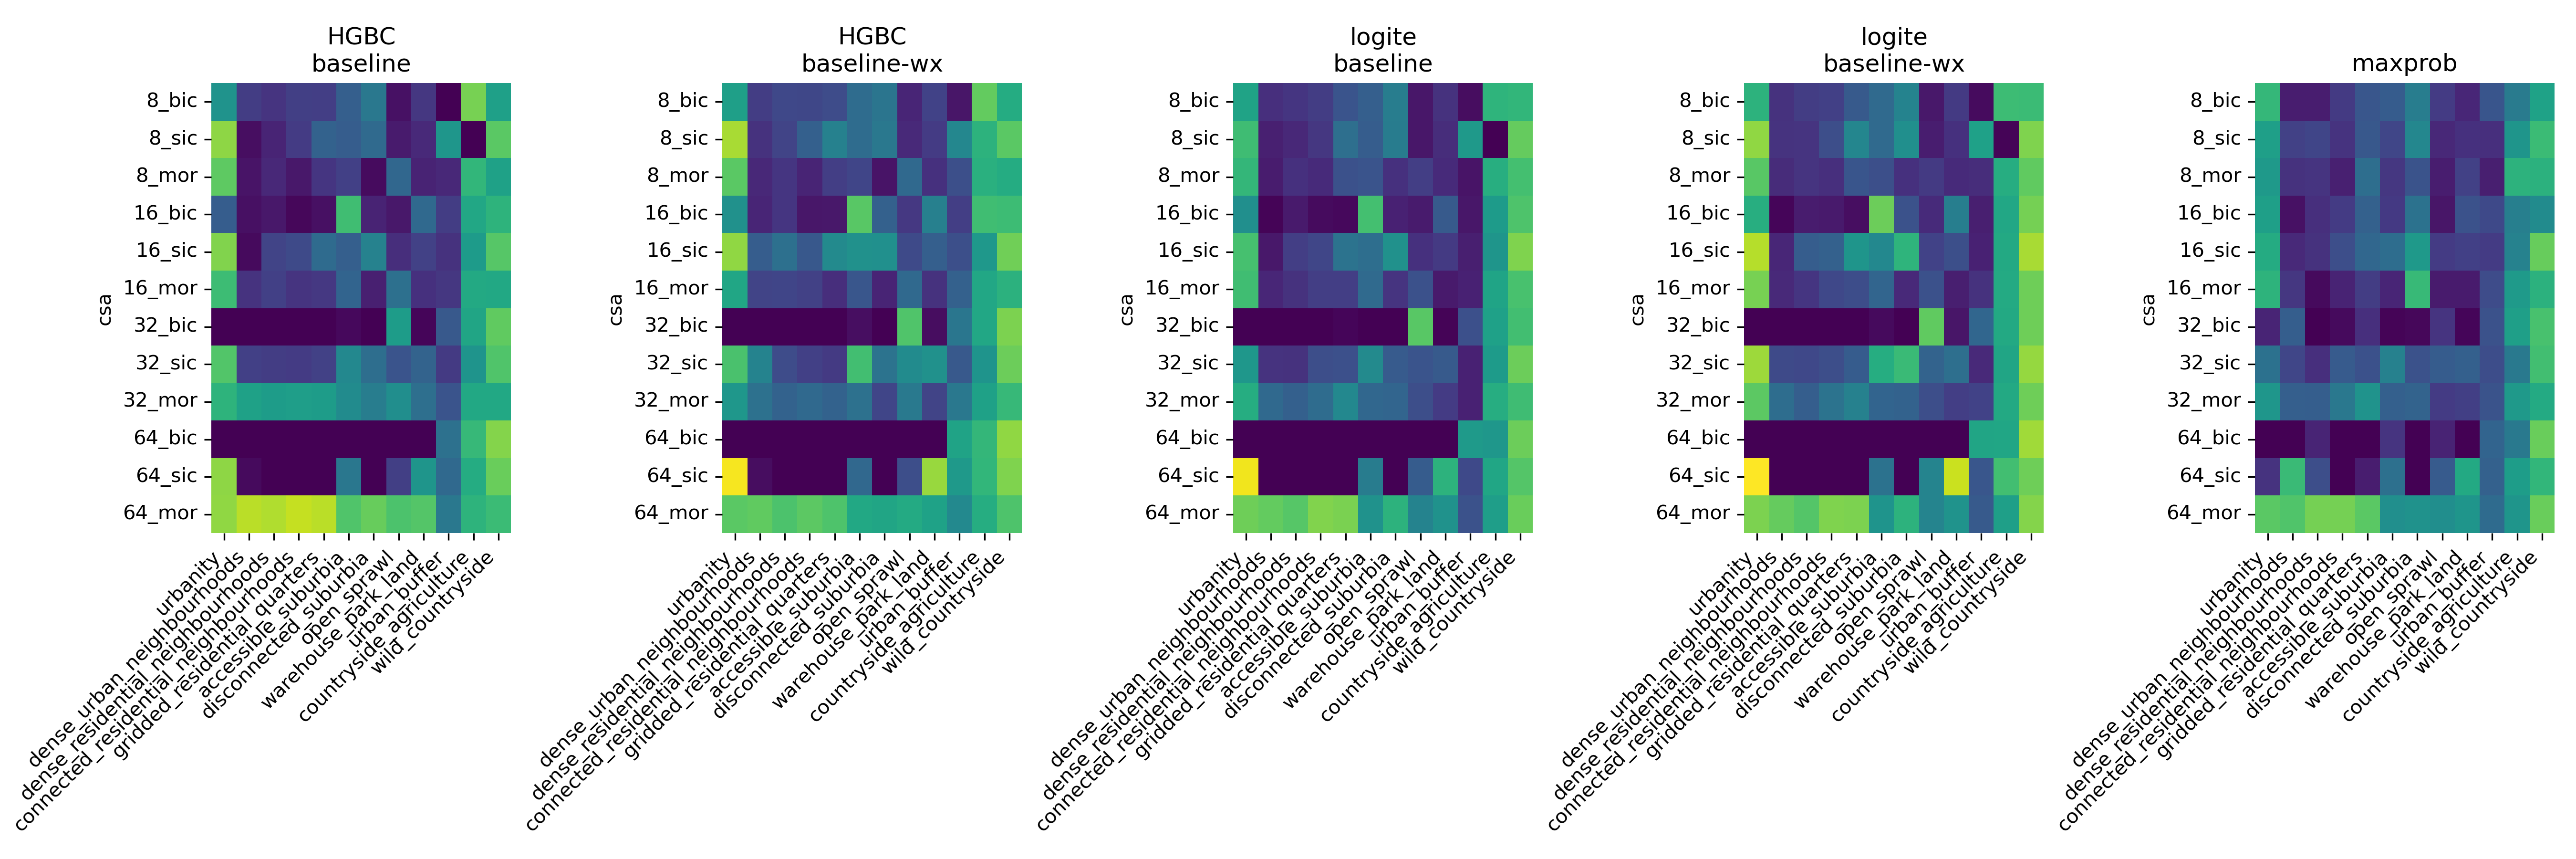
\includegraphics[width=1.0\linewidth]{fig/wc_accuracy_x_model.png}
%           \caption{\footnotesize TBC}
%           \label{fig:prediction_comparison_maps}
%       \end{figure}
% DAB: for space constraints, we have decided to drop it for now

The regression outputs explaining differences in the spatial pattern between observed
and predicted values measured by the Join Counts statistic offer another - spatially
explicit - perspective on the performance of tested model configurations. As such, it
also indicates slightly different results as presented in the table \ref{tab:sp_reg_wc}.
Neither option of the probability modelling steps seem to have a significant effect on
the Join Counts results, unlike in previous performance metrics. However, the
architecture of the neural network step shows a significant effect as multi-output
regression, and in two out of four cases also sliding image classification, outperform the
baseline image classification. While the effect of the chip size is inconsistent across the
options, the inclusion of the spatial lag in the modelling step has a significant effect (at
either 10\%, 5\% or 1\% significance level). The effect of a signature type depends on
its nature. More compact urban types like \textit{Urbanity} and \textit{Dense
urban neighbourhoods} show significance when using a distance threshold spatial weights,
while sparser signature types like \textit{Open Sprawl} and \textit{Urban Buffer} show
significance when using a union of weights.


% table 2 spatial,

\begin{table}
        \begin{tabular}{lcccc}
                \toprule
                {} &  $JC$ & $\log(JC)$ & $JC$  & $\log(JC)$  \\
                {} &  $W\_{thr}$ &  $W\_{thr}$ &  $W\_{union}$ &  $W\_{union}$ \\
                \midrule
                Intercept                                         &   4.3454*** &       1.4617*** &    4.7103*** &         1.6311*** \\
                                                                  &    (0.9507) &        (0.1344) &     (0.5763) &          (0.1080) \\
                (M) Logit E.                                      &     -0.1406 &         -0.0431 &       0.1851 &            0.0481 \\
                                                                  &    (0.4951) &        (0.0700) &     (0.2995) &          (0.0561) \\
                (M) Max. Prob.                                    &      0.1128 &         -0.1223 &       0.2819 &            0.0223 \\
                                                                  &    (0.6442) &        (0.0911) &     (0.3887) &          (0.0728) \\
                (A) M.O.R.                                        &  -3.1630*** &      -0.5744*** &   -2.7875*** &        -0.4647*** \\
                                                                  &    (0.5494) &        (0.0777) &     (0.3301) &          (0.0619) \\
                (A) S.I.C.                                        &      0.0119 &      -0.2390*** &    -0.6666** &           -0.0481 \\
                                                                  &    (0.5532) &        (0.0782) &     (0.3329) &          (0.0624) \\
                Chip Size                                         &   0.0297*** &         -0.0005 &      -0.0061 &        -0.0080*** \\
                                                                  &    (0.0108) &        (0.0015) &     (0.0065) &          (0.0012) \\
                W                                                 &    -0.9325* &       -0.1376** &   -0.9556*** &        -0.1785*** \\
                                                                  &    (0.4945) &        (0.0699) &     (0.2991) &          (0.0560) \\
                (S)Urbanity                                       &   4.6650*** &       0.6574*** &       0.1156 &           -0.1258 \\
                                                                  &    (1.0696) &        (0.1512) &     (0.6460) &          (0.1211) \\
                (S)Dense urban neighbourhoods                     &     1.7796* &       0.5094*** &       0.7480 &            0.1609 \\
                                                                  &    (1.0695) &        (0.1512) &     (0.6487) &          (0.1216) \\
                (S)Dense residential neighbourhoods               &     -0.8545 &          0.0672 &      -0.4636 &           -0.0920 \\
                                                                  &    (1.0958) &        (0.1550) &     (0.6647) &          (0.1246) \\
                (S)Connected residential neighbourhoods           &     -0.3656 &          0.1543 &      -0.4388 &           -0.1447 \\
                                                                  &    (1.1018) &        (0.1558) &     (0.6647) &          (0.1246) \\
                (S)Gridded residential quarters                   &     -0.2000 &          0.1009 &      -0.6203 &          -0.2111* \\
                                                                  &    (1.0744) &        (0.1519) &     (0.6517) &          (0.1221) \\
                (S)Disconnected suburbia                          &     -0.9752 &         -0.1719 &      -1.0303 &        -0.3358*** \\
                                                                  &    (1.1213) &        (0.1586) &     (0.6684) &          (0.1252) \\
                (S)Open sprawl                                    &     1.8342* &          0.1734 &    2.1575*** &         0.3576*** \\
                                                                  &    (1.0604) &        (0.1499) &     (0.6432) &          (0.1205) \\
                (S)Warehouse park land                            &      0.5496 &          0.2123 &      1.2245* &          0.3054** \\
                                                                  &    (1.0694) &        (0.1512) &     (0.6487) &          (0.1216) \\
                (S)Urban buffer                                   &     -0.0558 &         -0.0931 &    2.7027*** &         0.5164*** \\
                                                                  &    (1.0521) &        (0.1488) &     (0.6382) &          (0.1196) \\
                (S)Countryside agriculture                        &     -1.3759 &        -0.2511* &       0.6623 &            0.0670 \\
                                                                  &    (1.0521) &        (0.1488) &     (0.6382) &          (0.1196) \\
                (S)Wild countryside                               &    -2.0183* &      -0.5065*** &      -0.5918 &           -0.1635 \\
                                                                  &    (1.0521) &        (0.1488) &     (0.6382) &          (0.1196) \\
\midrule
                $R^2$                                             &      0.1589 &          0.1954 &       0.2118 &            0.2660 \\
                $R^2$ Adj.                                        &      0.1368 &          0.1743 &       0.1913 &            0.2468 \\
                N.                                                &      665    &      665        &   670        &     670           \\
                \bottomrule
                \end{tabular}
    \caption{\label{tab:sp_reg_wc}\footnotesize Regression outputs explaining
            (log of) differences in the spatial pattern between observed and predicted values,
            as measured by the Join Counts statistic. The Join Counts for each signature were computed
            using two types of spatial weights: one based on a distance threshold of 1Km ($W\_{thr}$),
            and another one built as a the union of nearest neighbor and queen contiguity matrices ($W\_{union}$).
            Explanatory variables with a preceding (M), (A) and (S)
    correspond to binary variables for the type of model (with histogram-based
            boosted classifier, or \texttt{HGBC}, as the
    baseline), architecture (with baseline image classification, or
    \texttt{BIC}, as the baseline) and spatial signature (with Accessible
    suburbia as the baseline),
    respectively. Standard errors in parenthesis. Coefficients significant at
    the 1\%, 5\%, 10\% level are noted with ***, **, and *, respectively.}
\end{table}



